\chapter{Preliminaries}
\label{chap:prelim}

Here, we introduce concepts, vocabulary terms, operations, and initial related work that is referenced throughout this dissertation.
The theme of each of these subject areas is the representation of information, whether that information relates to the operation of binary code, the content of removed text, or a deduced interpretation of an existing system.

\section{Abstract Interpretation}

Under the traditional definition, \emph{abstract interpretation} is a method of approximating the behavior of a program using monotonic functions over ordered sets (typically lattices).
It is related to the emulation of a program in that it is intended to extract a model of the program's behavior without performing the exact computations involved.
However, abstract interpretation has become more of a general framework for defining relations between different domains, as the necessity of translation between dissimilar symbolic representations, e.g. in transpilers, has become more prevalent.

Arbitrarily, let $L$ and $L'$ be \emph{concrete} and \emph{abstract} ordered sets, respectively.\footnote{The ordering of higher or lower levels of abstraction themselves is a function over the mathematical structures being discussed.}
These sets are related to each-other by a total function, which maps elements in one set to another.
We define two functions, $\alpha$ and $\gamma$, which map elements of $L$ to $L'$ and vice versa, and are called the \emph{abstraction} function and \emph{concretization} function respectively.

Then, given ordered sets $L_{1}, L_{2}, L'_{1}, L'_{2}$, the concrete semantics $f$ is a monotonic function from $L_{1}$ to $L_{2}$, and a correct abstraction from $L$ to $L'$ is \emph{valid} if the abstract semantics $f'$ mapping $L'_{1}$ to $L'_{2}$ preserves the ordering in $f$ of $L_{1}$ to $L_{2}$.
In this definition the function used to provide an order on objects in the sets is undefined.
The primary goal of abstract interpretation is to explore all executions of a program by over-approximation.
This is established by working from an abstraction of a concrete state (e.g. registers and memory) and providing commutativity: given a $c' = o(c)$ where $o$ is an operation and $c$ a concrete state, and $\alpha(c)$ the abstraction of $c$, $o(\alpha(c)) = \alpha(o(c))$ must hold true.
Second, states are \emph{joined} when their execution reaches an equivalent program counter (in the simplest case, by combining two sets, e.g. $a\ join\ b = \{a,b\}$).
They may also be \emph{widened}, a statement in logic which handles undecidable semantics, e.g. loops, to ensure all executions are ultimately analyzed.

\subsection{Symbolic Execution}

A standard misconception is that \emph{symbolic execution} is a form of abstract interpretation: symbolic execution is concerned with the expression of the values of all variables (the state) for arbitrary points in a program's execution as functions of initial values.
To do so, it only needs to compute an under-approximation of the possible program states, and not all possible executions.
However, in practice, symbolic execution is implemented \emph{through} a method for the abstract interpretation of a concrete, machine code program into the theory of bit-vectors.
For example, in standard execution the statement $(x > 5) ?\ y + 1 : x + 1$ would be concretely evaluated to 4 if $x = 3$, however, a standard symbolic execution, the system will record the pair $(x<=5; x=x+1),(x>5;x=y+1)$ into a symbolic state, representing the two possible execution paths.
Unlike abstract interpretation, symbolic execution's limitations make it more immediate: a function of initial values can be defined without explicit widening or joining operations.

Symbolic execution is a powerful tool for program analysis, but it is not without its limitations.
The core challenge is the \emph{path explosion} problem, where the number of possible execution paths grows exponentially with the number of branches in the program.
This can be limited through \emph{loop invariant} analysis, where the system attempts to identify the invariants of a loop and only execute the loop a finite number of times, a \emph{search strategy}, which determines which execution paths to explore from the exponential number possible, or a number of other deductive techniques.
Closely related is the challenge of \emph{memory aliasing}, which occurs when the system is unable to determine whether two pointers point to the same memory location, as the values of each pointer are treated as symbolic expressions over the theory of bit-vectors rather than concrete values.
Additionally, there is the \emph{environmental modeling} problem, where symbolic execution is unsound due to missing context, typically because the specific execution behavior of the hardware is not present, e.g. interrupts or highly-specific micro-architectural features.

\subsection{Lifting}
\label{ref:lifting-prelim}

We contrast abstract interpretation with the notion of \emph{lifting}, a borrowed term concept from category theory, where given a structure-preserving map from one mathematical structure to another of the same type (a morphism), $f: X \rightarrow Y$,  and another $g: Z \rightarrow Y$, a lifting of $f$ to $Z$ is a morphism $h: X \rightarrow Z$ such that $f = g \circ h$, or more simply, a function that points to another representation that \emph{may} more closely resemble the structure $Y$ but also has a morphism to $Y$ (Fig.~\ref{fig:lift}).

\begin{figure}[h]
\centering
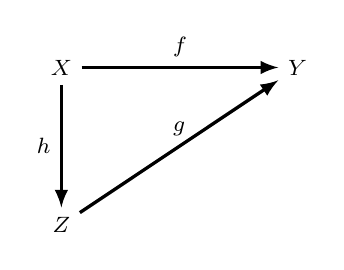
\begin{tikzpicture}[
  >=latex,
  every edge/.style={draw, very thick},
  every node/.style={font=\footnotesize},
  lift/.style={draw=none, fill=none}
  ]
  \node (X) at (0,0) {$X$};
  \node (Y) at (3,0) {$Y$};
  \node (Z) at (0,-2) {$Z$};
  \draw[->] (X) edge node[above] {$f$} (Y);
  \draw[->] (Z) edge node[above] {$g$} (Y);
  \draw[->] (X) edge node[left] {$h$} (Z);
\end{tikzpicture}
\caption{Lifting $f$ to $Z$}
\label{fig:lift}
\end{figure}

When applied to code, lifting typically refers to exposing the semantic structure of the binary to a higher level of abstraction.
However, as the mathematical definition suggests, lifting may also refer to a \emph{different} structure with the same morphism to the ``true'' structure.
Note that lifting is a form of \emph{translation}, but the new structure exists over a different domain.
For example, machine code may be lifted to a symbolic representation that represents a call-graph, or it may be lifted to a higher-level language, e.g. C, but it would be translation rather than lifting if the code was made into an equivalent, different machine code, e.g. ARM to x86.

Standard forms of lifting include translating a program into a form of graph representing latent relationships in the program, in order to simplify algorithms for reasoning about the program's structure.
For example, a program may be translated into a \emph{control flow graph} (CFG), where each node represents a basic block of code and each edge represents a possible transition between blocks.
Figure~\ref{fig:cfg} shows an example of lifting a CFG from a simple machine code program.

\begin{figure}[h]
\centering
\begin{tikzpicture}[
  >=latex
]
% split the picture into two halves. on the left have the disassembly and on the right the CFG
% disassembly with a simple branch
\node (disassembly) at (0,0) {
\begin{tabular}{ll}
\texttt{0x0} & \texttt{mov eax, 0x0} \\
\texttt{0x5} & \texttt{mov ebx, 0x1} \\
\texttt{0xa} & \texttt{cmp eax, ebx} \\
\texttt{0xc} & \texttt{jne 0x15} \\
\texttt{0xe} & \texttt{mov eax, 0x1} \\
\texttt{0x13} & \texttt{jmp 0x1a} \\
\texttt{0x15} & \texttt{mov eax, 0x0} \\
\texttt{0x1a} & \texttt{ret}
\end{tabular}
};
% CFG
\node (cfg) at (6,0) {
\begin{tikzpicture}[
  >=latex,
  every edge/.style={draw, very thick},
  every node/.style={font=\footnotesize},
  lift/.style={draw=none, fill=none},
  block/.style={draw, rectangle, minimum height=0.5cm, minimum width=0.5cm}
  ]
  \node[block] (0) at (-3,-2) {\texttt{0x0}};
  \node[block] (5) at (-1.5,-2) {\texttt{0x5}};
  \node[block] (a) at (0,-2) {\texttt{0xa}};
  \node[block] (c) at (0,-3) {\texttt{0xc}};
  \node[block] (e) at (0,-4) {\texttt{0xe}};
  \node[block] (13) at (0,-5) {\texttt{0x13}};
  \node[block] (15) at (-1.5,-6) {\texttt{0x15}};
  \node[block] (1a) at (0,-6) {\texttt{0x1a}};
  \draw[->] (0) edge (5);
  \draw[->] (5) edge (a);
  \draw[->] (a) edge (c);
  \draw[->] (c) edge (e);
  \draw[->] (e) edge (13);
  \draw[->] (15) edge (1a);
  \draw[->] (c) edge[bend right=30] (15);
  \draw[->] (13) edge (1a);
\end{tikzpicture}
};
% draw an arrow between the two halves
\draw[->, very thick] (disassembly) edge (cfg);
\end{tikzpicture}
\caption{Lifting a CFG from machine code}
\label{fig:cfg}
\end{figure}

\emph{Program slicing} is a form of lifting which transforms a program specification into \emph{slices}, sets of statements affecting sets of values in the program's state at some points of interest.
More generally, they may also refer to arbitrary subsets of the program's statements.
The determination of the slices is typically referred to as a \emph{slice criterion}.
Symbolic execution can be used to determine a given slice by exploring all paths through a program and thus the statements which affect the value of a variable of interest.

\subsection{Intermediate Representations}

The term \emph{intermediate representation} (IR) refers to a representation of a program that is used as an intermediate step of a translation process, typically for a compiler.
The IR is typically designed to be easy to translate to and from the source and target languages, and to be easy to reason about.
Referring to Fig.~\ref{fig:lift}, in lifting the IR is the structure $Z$ used to translate between $X$ and $Y$.
The critical form of IR for use in symbolic execution and abstract interpretation more generally are abstract syntax trees (ASTs).
ASTs are a form of IR that represent the syntactic structure of a program as a tree, where each node represents a syntactic construct and each edge represents a relationship between constructs.
For example, the AST for the expression \texttt{a + b * c} is shown in Fig.~\ref{fig:ast}.

\begin{figure}[h]
\centering
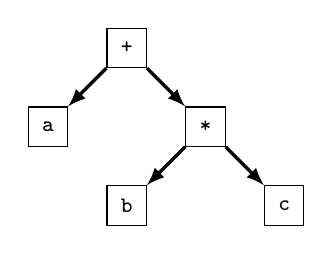
\begin{tikzpicture}[
  >=latex,
  every edge/.style={draw, very thick},
  every node/.style={font=\footnotesize},
  lift/.style={draw=none, fill=none},
  block/.style={draw, rectangle, minimum height=0.5cm, minimum width=0.5cm}
  ]
  \node[block] (plus) at (0,0) {\texttt{+}};
  \node[block] (a) at (-1,-1) {\texttt{a}};
  \node[block] (times) at (1,-1) {\texttt{*}};
  \node[block] (b) at (0,-2) {\texttt{b}};
  \node[block] (c) at (2,-2) {\texttt{c}};
  \draw[->] (plus) edge (a);
  \draw[->] (plus) edge (times);
  \draw[->] (times) edge (b);
  \draw[->] (times) edge (c);
\end{tikzpicture}
\caption{AST for \texttt{a + b * c}}
\label{fig:ast}
\end{figure}

% relate IRs to Hoare Logic. Is Hoare Logic an IR?
ASTs may be used in conjunction with \emph{Hoare logic} to reason about programs.
Hoare logic is a formal system for reasoning about the correctness of programs.
It is based on the notion of \emph{Hoare triples}, which are statements of the form $\{P\} S \{Q\}$, where $P$ and $Q$ are \emph{predicates} and $S$ is a statement.
The meaning of a Hoare triple is that if the predicate $P$ holds before the execution of $S$, then the predicate $Q$ will hold after the execution of $S$.
For example, the Hoare triple $\{x = 0\} x := x + 1 \{x = 1\}$ states that if $x$ is equal to $0$ before the execution of $x := x + 1$, then $x$ will be equal to $1$ after the execution of $x := x + 1$.

This is equivalent to a \emph{satisfaction relation} between a program and a specification, which evaluates to true if the program satisfies the specification.
In symbolic execution, this specification is represented as a set of predicates defined over the program's state, determined both by external inputs and the current execution path under consideration.
By evaluating the satisfaction relation, symbolic execution can determine whether a given path is feasible.

Finally, note that while symbolic execution, lifting, and intermediate representations \emph{can} preserve a program's semantics, each has the potential to introduce errors.
For example, the process of lifting a program to an IR may introduce errors if the IR is not expressive enough to represent the semantics of the program.
The outputs of this translation ultimately serve to perform analysis on the program's behavior, and the correctness of this analysis depends on the correctness of the translation.
Thus, the use of these techniques is ultimately one basis for emulation, an insight that will become more apparent in our discussion of QEMU (Sec.~\ref{sec:hardemu}).

\section{Information}

Many definitions of \emph{information} exist---this dissertation will use information to represent \emph{pure difference} or distiguishability between two objects, e.g. 0 and 1.
A key measure of information is \emph{entropy} which quantifies the amount of uncertainty involved in a random process~\cite{cover1999elements}.
Given a discrete random variable $X$ with a probability distribution $P$, the entropy of $X$ is defined as

\begin{equation}
H(X) = -\sum_{x \in X} P(x) \log_2 P(x)
\end{equation}

\noindent
where $P(x)$ is the probability that $X$ takes on the value $x$.
For example, the entropy of a fair coin is $H(X) = -\frac{1}{2} \log_2 \frac{1}{2} - \frac{1}{2} \log_2 \frac{1}{2} = 1$.
The entropy of a biased coin with $P(\text{heads}) = 0.9$ is $H(X) = -0.9 \log_2 0.9 - 0.1 \log_2 0.1 \approx 0.47$.
The use of base 2 for the log indicates that entropy is measured in \emph{bits}.
Entropy quantifies the amount of information in a distribution as the number of bits required to represent it.
For a uniform distribution over $n$ values, the entropy is $\log_2 n$.

It is therefore also possible to quantify the amount of information \emph{leaked} by a random process $f$ taking a ``secret'' input $X$ and producing output $Y$ as what number of bits of $X$ may be inferred from $Y$.
If the number of bits determinable from $Y$ about $X$ is lower than the total number of bits required to represent $X$, information has been lost.
This does not necessarily indicate it is impossible to disambiguate a \emph{specific} value using accessible information, but (assuming quantization) that some value from the initial distribution cannot be differentiated from some other value.

For accurate emulations and measuring security, we are concerned with determining how much information it is possible to recover about $X$ from $Y$.
However, $X$ is inaccessible in many cases, so we must select some $X'$ as a \emph{dictionary} limiting the scope of the possibilities we are willing to consider.
Selecting a point $x \in X'$, if $f(x) \in Y$ and $f$ is assumed deterministic, then it is possible $x \in X$.
In some cases it is possible to construct a dictionary that is \emph{complete}, i.e. that contains all possible values.
When a dictionary is incomplete, often due to practical limitations on computation and analysis time, it becomes necessary judge whether a dictionary is reasonable.

\subsection{Guess-and-Check}

We consider a dictionary reasonable if it contains values that are likely to be observed in practice.
However, this is not a sufficient restriction for \emph{soundness}, i.e. that results derived from considering the dictionary as the superset of the accessible information must include all correct values.
So we have two forms of uncertainty: analytic uncertainty with respect to the dictionary, and empirical uncertainty with respect to the resolution of the correct dictionary entry from available information.
The former occurs in cases where the true set of values may not be a strict subset of the considered values, and the latter occurs where information is lost.

The derivation of a value from accessible information is a \emph{guess} and must be subject to some form \emph{check}, or \emph{oracle} to determine whether, in fact, it is a correct derivation.
However, when analyzing real systems, an oracle is often unavailable, so we must rely on the statistical probability of a guess being correct.

\subsection{Regularity Conditions, Dependence, and Independence}

Correct guesses are dependent on certain \emph{regularity conditions}, assumptions which imply a given estimation of a probability is correct.
For example, assuming a \emph{uniform} distribution over a set of values implies that the probability of any value being selected is equal to the inverse of the number of values.
In contrast, an \emph{empirical} distribution over a set of values implies that the probability of any value being selected is equal to the frequency of that value in the set.

The probability of a guess being correct is dependent on the amount of information available to the guesser, and is informed by the method of analysis.
We therefore differentiate between \emph{dependent} and \emph{independent} information.
Two pieces of information are \emph{dependent} if the presence of one piece of information affects the probability the other is also present.
Two pieces of information are \emph{independent} if the presence of one piece of information does not affect the probability of the other being present.

In this dissertation, we will consider the role that the probability a guess is correct plays when measuring security and constructing emulations.
Our study of rehosting will demonstrate perfect inference of an absolutely ``correct'' value returned by a missing hardware device is not necessary to construct a useful emulation.
In studying redactions, we will show how assuming a certain regularity condition, e.g. an empirical distribution of names in a population, can make privacy attacks significantly more effective.
Finally, our framework for the extraction of continuous functions from binary firmware will illustrate the utility of frameworks for inferring and explicating dependencies between information in a system.
